\subsection{Switch Sensors Attack}

This attack is performed by adding a \code{sensor\_attack} function to the
\code{controller} FMU\@.

The attacker can tune the following parameters:
\begin{itemize}
	\item \code{Real attack\_time}: The time at which the attack starts.
	\item \code{Real attack\_duration}: The duration of the attack.
	\item \code{Bool cyclic}: If \code{true} the attack is performed
		periodically.
\end{itemize}

The attack switches the right and left sensors' output, as we can see from
\lstref{lst:switchsensorsatk}.

\lstinputlisting[language=C, label={lst:switchsensorsatk},
caption={Switch sensors attack function}]{switch-sensors-attack-control.c}

We can see from \figref{fig:switchsensorsatkresult} that, when the attack
starts, the robot rotates to the right and gets away from the path. After that,
the robot continues to rotate since it cannot see any line to the right nor to
the left. When the attack ends, the robot manages to get back to the correct
path when it hits against the line again.

\begin{figure}[htb]
	\centering
	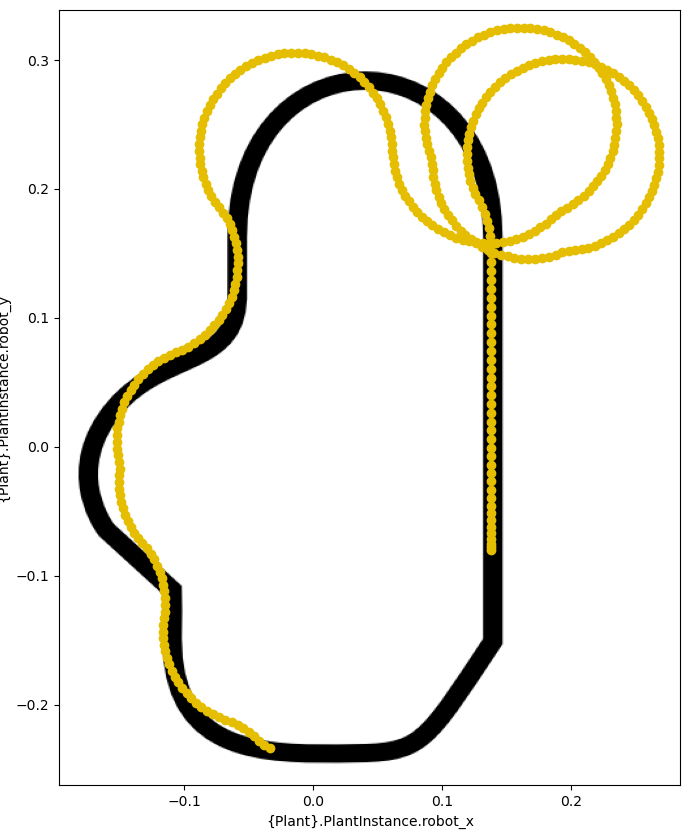
\includegraphics[width=0.43\textwidth]{switch-sensors-attack}
	\caption{Line follower robot path when
	attacked}\label{fig:switchsensorsatkresult}
\end{figure}
